\section{Tipos de sistemas operativos}
Los sistemas operativos pueden clasificarse de diversas maneras, por la administración de usuarios, administración de tareas, manejo de recursos, entorno de destino, entre otros criterios. En esta sección se abordarán específicamente las siguientes clasificaciones: sistemas operativos monousuario y multiusuario, monotarea y multitarea, de tiempo real (RTOS), distribuidos, móviles y embebidos. A continuación, el análisis de dichas clasificaciones.

\subsection{Monousuario vs. Multiusuario}
Estos tipos de sistemas operativos, son resultado de una clasificación por la cantidad de usuarios que los operan.  

\textbf{Monousuario:} Como su nombre hace evidente, fue planificado para usar la computadora de forma que solo una persona a la vez lo haga correctamente, esto no significa necesariamente que solo pueda hacer una tarea a la vez \citep{kaur2022osreview}. Sin embargo y completando el concepto, en la práctica más de una persona puede usarlo debido a que el sistema operativo no distingue entre personas \citep{olivares2021sohardware}. Según \citep{kaur2022osreview}, algunos ejemplos resaltantes de sistemas operativos monousuario son Palm OS y Windows (versiones antiguas).  

\textbf{Multiusuario:} Este tipo de sistema, hace posible que varios usuarios usen el computador de manera simultánea, para lo cual el sistema operativo debe administrar los recursos de manera adecuada; es necesario distinguir sistemas operativos multiusuario de sistemas monousuario compatibles con redes, en los cuales el único usuario “real” es el administrador \citep{kaur2022osreview}; otra característica del tipo multiusuario es distinguir entre las personas (usuarios) que acceden a la computadora \citep{olivares2021sohardware}. Según \citep{kaur2022osreview} complementado por \citep{olivares2021sohardware} y \citep{kabiraj2018oscase}, algunos ejemplos resaltantes de sistemas operativos multiusuario son Windows 7, Windows 10, UNIX, LINUX, VMS y el sistema operativo de servidor MVS.  

\subsection{Monotarea vs. Multitarea}
Estos tipos de sistemas operativos, son resultado de una clasificación por la administración de la ejecución de tareas.  

\textbf{Monotarea:} Como indica su raíz griega, solo hacen una tarea a la vez. En la actualidad están casi en completo desuso, debido a que no aprovecha de manera óptima los recursos. Un ejemplo resaltante de sistema operativo multitarea es MS-DOS, el cual actualmente se encuentra en desuso \citep{olivares2021sohardware}.  

\textbf{Multitarea:} Estos sistemas operativos son capaces de ejecutar varias tareas a la vez, y por ello maximizan el uso de los recursos de la computadora. Además, también algunos sistemas operativos para móviles son multitarea. Los sistemas operativos multitarea, a su vez se pueden clasificar por su forma de administrar el tiempo de ejecución de sus aplicaciones en: Sistemas de tiempo compartido y sistemas de tiempo real \citep{olivares2021sohardware}. Según \citep{rawat2025osstudy} algunos ejemplos resaltantes de sistemas operativos multitarea son Windows 10/11, Linux, Unix, macOS.  

\subsection{Tiempo real (RTOS)}
Los sistemas operativos de tiempo real son un tipo de sistema operativo multitarea. Mientras que su contraparte, los sistemas de tiempo compartido, se aprovechan del uso de pequeños intervalos de tiempo, para asignarlos a la ejecución de cada programa (time slice) y cambiar rápidamente entre las ejecuciones de estos programas (context switch), dando así la sensación de paralelismo; los sistemas operativos de tiempo real, no poseen intervalos de tiempo para definir la ejecución de un programa, sino que el programa se ejecuta hasta que termine (y dicho tiempo está definido también en el programa) o hasta que un programa de mayor prioridad lo interrumpa \citep{olivares2021sohardware}.  

En la actualidad se usan mayormente los sistemas operativos de tiempo compartido, pero los sistemas operativos de tiempo real juegan un papel clave en campos que requieran precisión en cuanto al tiempo de procesamiento como medicina, tráfico aéreo, plantas de energía, entre otros \citep{olivares2021sohardware}.  

En síntesis, estos sistemas buscan precisión en la sincronización, a partir de respuestas predecibles (determinismo) y se pueden clasificar de acuerdo a su tolerancia a errores en RTOS duros y RTOS suaves. Algunos ejemplos resaltantes son VxWorks, FreeRTOS y QNX \citep{rawat2025osstudy}.  

\subsection{Distribuidos}
Los sistemas operativos distribuidos controlan múltiples nodos independientes como si fueran un solo sistema, varios computadores en red ejecutan conjuntamente un OS único, de modo que el usuario percibe una sola computadora con hardware extra. Cada nodo corre un núcleo mínimo y componentes de gestión que intercomunican y comparten recursos con el objetivo de lograr transparencia (single-system image) \citep{garg2013dos}. Algunos ejemplos resaltantes son Google Fuchsia OS y Solaris OS \citep{rawat2025osstudy}.  

\begin{figure}[H]
    \centering
    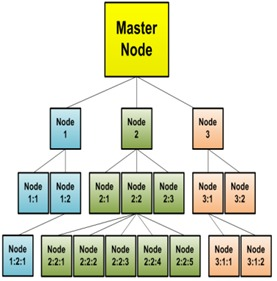
\includegraphics[width=0.4\textwidth]{figures/distributedSistems.jpg}
    \caption[Organización de nodos en un sistema operativo distribuido]%
            {Organización de nodos en un sistema operativo distribuido \citep{garg2013dos}}
    \label{fig:distributed_os}
\end{figure} 

\subsection{Móviles}
Los sistemas operativos móviles se diseñan para teléfonos inteligentes, tabletas y otros dispositivos portátiles táctiles, tiene como característica ser bastante intuitivos, ligeros y con un enfoque hacia el ahorro de la batería. Además, admiten funciones avanzadas en tecnología como interacción táctil, comunicación inalámbrica y ejecución de diversas aplicaciones. Algunos de los ejemplos más resaltantes son Android OS e iOS \citep{rawat2025osstudy}.  

A continuación, una línea de tiempo de la evolución de los sistemas operativos móviles:  

\begin{figure}[H]
    \centering
    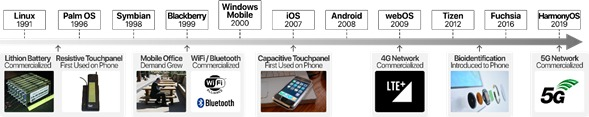
\includegraphics[width=1.0\textwidth]{figures/timeLineMobile.jpg}
    \caption[Desarrollo cronológico de los sistemas operativos móviles y hitos tecnológicos asociados]
            {Desarrollo cronológico de los sistemas operativos móviles y hitos tecnológicos asociados \citep{jia2024acos}}
    \label{fig:mobile_os}
\end{figure} 

\subsection{Embebidos}
Los sistemas operativos embebidos son diseñados para satisfacer los requerimientos específicos de los sistemas embebidos, son aplicados en diversos campos, tales como electrodomésticos, controles remotos e incluso instrumentos aeroespaciales. No requieren de demasiados recursos como energía, memoria ni espacio de almacenamiento; y aún así son capaces de brindar eficiencia y precisión, además de un nivel de personalización bastante alto para hacerlos funcionar en situaciones difíciles y cambiantes \citep{jia2024acos}. Algunos de los ejemplos más resaltantes son Embedded Linux y Windows Embedded Compact \citep{rawat2025osstudy}.  

A continuación, una línea de tiempo de la evolución de los sistemas operativos embebidos:  

\begin{figure}[H]
    \centering
    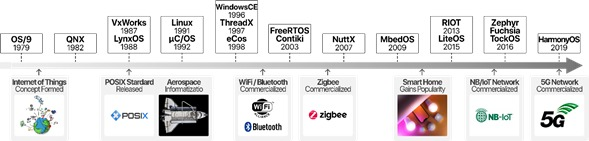
\includegraphics[width=1.0\textwidth]{figures/timeLineEmbeded.jpg}
    \caption[Desarrollo cronológico de los sistemas operativos embebidos y hitos tecnológicos asociados]
            {Desarrollo cronológico de los sistemas operativos embebidos y hitos tecnológicos asociados \citep{jia2024acos}}
    \label{fig:Embedded_os}
\end{figure} 

\subsection{Comparación entre tipos de Sistemas Operativos}

\begin{munltab}{|c|p{8cm}|p{8cm}|}
  {comparacion_tipos_so}
  {Comparación de tipos de sistemas operativos basado mayormente en \citep{rawat2025osstudy}}
\hline
\textbf{Tipo de SO} & \textbf{Ventajas} & \textbf{Desventajas} \\
\hline
Monousuario & Simplicidad en diseño y administración, adecuado para uso personal & No diferencia usuarios, limitaciones en entornos colaborativos \\
\hline
Multiusuario & Permite que múltiples usuarios accedan simultáneamente, gestión de recursos más avanzada & Mayor complejidad en seguridad y administración de cuentas \\
\hline
Monotarea & Implementación sencilla, bajo consumo de recursos & No aprovecha el hardware moderno, ineficiente y obsoleto \\
\hline
Multitarea & Aprovecha mejor los recursos, permite ejecución paralela de procesos & Complejidad en la gestión de concurrencia y planificación \\
\hline
Tiempo Real (RTOS) & Respuestas deterministas, precisión crítica en aplicaciones sensibles (medicina, aeroespacial, etc.) & Difícil de implementar, requiere hardware confiable y costoso \\
\hline
Distribuidos & Transparencia de recursos, escalabilidad, tolerancia a fallos & Complejidad en diseño, comunicación entre nodos y sincronización \\
\hline
Móviles & Interfaz intuitiva, eficiencia energética, portabilidad & Limitados en recursos frente a sistemas de escritorio, dependencia de ecosistema cerrado \\
\hline
Embebidos & Alta eficiencia y personalización, bajos requerimientos de hardware & Poco flexibles, difíciles de actualizar y mantener \\
\hline
\end{munltab}